\documentclass[conference]{IEEEtran}
\IEEEoverridecommandlockouts
\usepackage{amsmath,amssymb,amsfonts}
\usepackage{amsmath}
\usepackage{algorithmic}
\usepackage{alltt}
\usepackage[noend]{algorithm2e}
\usepackage{amssymb}
\usepackage[style=ieee]{biblatex}
\usepackage{breakurl}
\usepackage{circuitikz}
\usepackage{caption}
\usepackage{colortbl}
\usepackage{color}
\usepackage{enumerate}
\usepackage{enumitem}
\usepackage{epstopdf}
\usepackage{flushend}
\usepackage{graphicx}
\usepackage[hidelinks]{hyperref}
\usepackage[utf8]{inputenc}
\usepackage{multirow}
\usepackage{pbox}
\usepackage{pgfplots}
\usepackage{picinpar}
\usepackage{pifont}
\usepackage{siunitx}
\usepackage{soul}
\usepackage{subcaption}
\usepackage{tabularx}
\usepackage{textcomp}
\usepackage{tikz} 
\usepackage{url}
\usepackage{xcolor}
%\usepackage{etoolbox}
%\patchcmd{\thebibliography}{\section*{\refname}}{\section*{\refname}\vspace{-1000em}}{}{}

\def\BibTeX{{\rm B\kern-.05em{\sc i\kern-.025em b}\kern-.08em
    T\kern-.1667em\lower.7ex\hbox{E}\kern-.125emX}}
\usetikzlibrary{shapes.geometric, arrows}
\usetikzlibrary{calc}
\usetikzlibrary{backgrounds}
\usetikzlibrary{patterns}
\usetikzlibrary{decorations.pathreplacing}
\addbibresource{Ref.bib}

\makeatletter
\newcommand{\removelatexerror}{\let\@latex@error\@gobble}
\makeatother

\usetikzlibrary{arrows.meta, fit}
\usepackage{booktabs}
% arguments are:  name caption content position color
\NewDocumentCommand\mytableat{m m +m m m}{%
    % main node, will contain the table
    \node [shape=rectangle,fill=#5, align=center](#1-t) at (#4) {
        \begin{tabular}{lc} \toprule
            #3
            \bottomrule
        \end{tabular}
    };
    \node [align=center, anchor=south](#1-c) at (#1-t.north) {#2};
    % this is the node encompassing both --- use inner sep to create
    % a white "space" around it
    \node [fit=(#1-t) (#1-c), inner sep=3mm](#1){};
}

\begin{document}

%\title{Algorithmic approach on the extraction of power flow configurations for multiport DC-DC converters\\
\title{Algorithmic Extraction of Power Flow Configurations for Three-Port DC-DC Converters\\

\thanks{The present work was financially supported by the Andreas
Mentzelopoulos Foundation (Corresponding Author: G.S.).}
}

\author{\IEEEauthorblockN{Georgios Salagiannis}
\IEEEauthorblockA{\textit{Department of Electrical and Computer Engineering} \\
\textit{University of Patras}\\
Patras, Greece \\
gsalagiannis@ac.upatras.gr}
\and
\IEEEauthorblockN{Emmanuel Tatakis}
\IEEEauthorblockA{\textit{Department of Electrical and Computer Engineering} \\
\textit{University of Patras}\\
Patras, Greece \\
e.c.tatakis@ece.upatras.gr}
}

\maketitle

\begin{abstract}
During the last two decades, power flow graphs have been established as a systematic and straightforward method for the design of DC-DC power converters. Several researchers have focused their efforts on the design of Three-Port Converters with this method for the integration of renewable energy sources, energy storage systems and DC micro-grids. However, even though all attempts utilize the same design method with slightly different application specifications (ESS existence, output bidirectionality, etc.), there is currently no attempt to group all the available power flow configurations under one procedure. This gap is addressed in this paper, where a systematic and algorithmic method is proposed to automatically derive all DC-DC converter power flow configurations, based on rule application and a single-variable user input. This work not only highlights the fundamentals of the power flow graph design while automating it, but also sets the ground for further study and optimization of a plethora of different configurations, without the restrictions posed by traditional manual design.
\end{abstract}

\begin{IEEEkeywords}
DC-DC Converters, Graph-Theory, Renewable Energy, Power Flow Graphs, Three-Port Converters
\end{IEEEkeywords}

\section{Introduction}
The Power Flow Graph (PFG) converter design was introduced by \cite{tse_theoretical_2000}. Initially, it was used to systematically derive converter topologies for Power Factor Correction (PFC), where an Energy Buffer (EB) was used. This led to the invention of Reduced Redundant Power Processing ($R^2P^2$) converters, which were Three Port Converters (TPCs), interconnected through basic converters. The main idea was that by changing the wiring configuration of those converters, higher system efficiency compared to a cascaded connection could be achieved. 

This design approach can be implemented in a plethora of applications, where the analysis based on power flow graphs applies. Yang et al. \cite{yang_synthesis_2015} utilized the $R^2P^2$ concept and power flow graphs to systematically examine and derive new topologies for Double Input Single Output (DISO) DC-DC converters. The researchers distinguish two cases; a) both inputs are voltage sources and b) one input is a voltage source and the other one is an Energy Storage System (ESS). For both cases, only the graph configurations allowing simple interconnections (meaning that at least one Type I sub-graph is existent) are discussed. For the circuit implementation, unidirectional (bidirectional) basic converters (buck, boost and buck-boost) are used for the first (second) case. The primary evaluation criterion is the efficiency of the overall system. 

Provided the increasing interest for DC-DC converters with high step-up capability, Palomo et al. \cite{loera-palomo_family_2015} 
attempted to design converters with quadratic voltage boosting with non-cascaded configurations, in order to address the inherently low efficiency of the cascaded quadratic boost family of converters. In this work, the TPC consists of an input, an EB and an output port, and only unidirectional basic converters are considered. Two fundamental contributions are made to the field; a) the developed configurations are systematically compared based on the graph configuration inherent gain and b) the concept of topology simplification and switch number minimization in $R^2P^2$ is introduced. Notably, only Types I-II and I-III are examined, owing to their wide conversion ratio.

Regardless of the previous efforts, a study and record of all possible $R^2P^2$ configurations and their suitability for high step-up applications was nonexistent. Therefore, this gap was filled by \cite{zogogianni_non-isolated_2019}, for converters with an input, an EB and an output port. All potential configurations were examined for converters composed of non isolated unidirectional basic converters and both their efficiency and voltage gain were derived.

During last decade, distributed power generation and DC Microgrids have emerged as a promising solution towards energy sustainability. In this direction, hybrid integration of RES and ESS is required, which has led to the development of TPCs with controlled storage port (opposite to the previous attempts with EB) \cite{salagiannis_review_2024}. Instead of a Single Input Single Output (SISO) converter for each component, a unified converter is used.  In \cite{aljarajreh_synthesis_2021}, based on the idea that TPCs can be composed from basic converters, power flow graphs are used to create and analyze TPCs for DC Microgrid applications. Specifically, two bidirectional ports are considered, namely the ESS and the output DC Bus. Opposite to \cite{zogogianni_non-isolated_2019}, the storage port is not considered as an EB freely satisfying power conservation, but rather as a fully controlled ESS. This leads to the utilization of both unidirectional and bidirectional converters. However, no efficiency or gain analysis is performed.


\begin{table*}
	%\renewcommand{\arraystretch}{1.3}
	%\caption{Units for Magnetic Properties}
	\centering
	\caption{Literature Review on PFG Three-Port DC-DC Converter Design.}
\label{tab:summary}
	%\resizebox{\columnwidth}{!}{
%\begin{tabular}{| m{69pt} || m{20pt} | m{30pt}| m{30pt} | m{35pt}||} 
\begin{tabularx}{\linewidth}{| c || c | c| c | X ||} 
         \hline
         \textbf{Researchers} & \textbf{Year} & \textbf{\#Ports} & \textbf{\# $\leftrightarrow$ Ports} & \textbf{Contribution}\\ [0.5ex] 
         \hline\hline 
         Tse et al. & 2001 & 3 & 1 &  Systematic study of power supplies with integrated PFC capability as TPCs, using power flow graphs and unidirectional fundamental converters.\\[0.5ex]
         \hline 
         Yang et al. & 2015 & 3 & 1 & Systematic study of TPCs with no or one bidirectional port (ESS), using power flow graphs and unidirectional/bidirectional fundamental converters.\\ [0.5ex]
         \hline 
         Palomo et al. & 2015 & 3 & 1 & Derivation of non-cascaded high step-up DC-DC converters, using power flow graphs and unidirectional fundamental converters.\\ [0.5ex]
         \hline
         Zogogianni et al. & 2019 & 3 & 1 & Systematic study of TPCs with one bidirectional port (Energy Buffer), using power flow graphs and unidirectional fundamental converters.\\[0.5ex]
         \hline 
         Aljarajreh et al. & 2021 & 3 & 2 & Systematic study of TPCs with two bidirectional ports (ESS and Output), using power flow graphs and unidirectional/bidirectional fundamental converters.\\ [0.5ex]
         \hline 
         Proposed & 2024 & 3 & 1-2 & Algorithmic derivation of power flow configurations for TPCs with EB and TPCs with ESS and unidirectional or bidirectional output, using both unidirectional and bidirectional converters.\\ [0.5ex]
         \hline
         \hline
\end{tabularx}
\end{table*}

The current status of the research on the field of PFG Three-Port DC-DC converter design is summarized in Table \ref{tab:summary}. It becomes apparent that even though some systematic derivation methods are described, there is no universal method to cover all possibilities (TPC with EB, TPC with ESS bidirectional port and TPC with bidirectional ports for ESS and output). Furthermore, manual effort is required to derive and examine all available power configurations, and therefore some studies are only focused on the graphs incorporating simple interconnections. In this paper, those issues are addressed by developing a programmable method for the derivation of Three-Port DC-DC converters with different features, based on the input provided by the user. Based on that, the contributions of this paper are summarized as follows:
\begin{itemize}
    \item It presents a coherent way to translate the traditional drawn power flow graphs to matrices that can be processed by a PC, so that the digital forms of PFGs with FCs can be generated.
    \item It proposes a universal and programmable method for the derivation of power flow configurations of TPCs that permits the design of any relevant converter only by changing certain parameters.
    \item It demonstrates and implements the algorithmic rationale for TPC converter design, summarizing previous works and providing useful insight to the researchers.
    %\item Having overcome the limitations of manual study, this method can be combined with future optimization studies, to extract fitting topologies for specific applications.
\end{itemize}


\section{Background for PFG Converter Design}
As described above, converters' PFG design is based on the idea that simple converters can be interconnected in a way that only part of the total power is processed through them. To concisely demonstrate various interconnection options, the power flow graphs were proposed. Based on the nature of its source or load, a port can either exclusively receive or offer power if it is unidirectional, or both if it is bidirectional. Furthermore, one port may offer (receive) power to (from) multiple ports. As shown in Fig. \ref{fig:power_port_types}, \textbf{Type I} is when power is transferred from one port to another, \textbf{Type II} is when two ports provide power to a third port and \textbf{Type III} is when a port provides power to the other two ports.  
\begin{figure}[htbp]\begin{minipage}{\columnwidth}\centering
        \begin{subfigure}{0.3\columnwidth}\centering
         \begin{circuitikz}[american voltages]
    \draw[->] (1, 0) -- (2,0);
\end{circuitikz}\caption{Type I}
        \end{subfigure}\hfill
        \begin{subfigure}{0.3\columnwidth}\centering
        \begin{circuitikz}[american voltages]
    \draw[->] (1,0) -- (2, 0);\draw[->] (2, 1) -- (2,0);\draw[->] (2,0)--(3,0);
\end{circuitikz}
        \caption{Type II}\end{subfigure}
        \begin{subfigure}{0.3\columnwidth}\centering
        \begin{circuitikz}[american voltages]
    \draw[->] (1,0) -- (2, 0);\draw[->] (2, 0) -- (2,1);\draw[->] (2,0)--(3,0);
\end{circuitikz}
        \caption{Type III}\end{subfigure}
        \caption{The Three Available SG Types.}\label{fig:power_port_types}\end{minipage}
\end{figure}
These SubGraphs (SGs) are combined to indicate all the power flow paths in a TPC, forming the complete PFG. Each arrow indicating power flow from (to) one port to (from) the SG will be called power flow vector from now on. For the case of a converter with input, EB and output ports, the complete power flow graph of Type I-IIA is shown in Fig. \ref{fig:I-IIA_graph} as an example. In the next design step, simple converters that will be called Fundamental Converters (FCs) from now on and will be denoted by lowercase letters a, b, etc., are interfered on the PFGs to achieve power flow controllability (Fig. \ref{fig:complete_graph}). 

\ctikzset{resistors/scale=0.6, % smaller R
capacitors/scale=0.7, % even smaller C
sources/scale=0.7 % small diodes
}
\begin{figure}[htbp]\begin{minipage}{\columnwidth}\centering

        \begin{subfigure}{0.45\columnwidth}\centering
         \begin{circuitikz}[american voltages]

    % Voltage source and capacitor on the left
    \draw (1,2) to[V] (1,1);\draw (1,1) -- (1.5,1);\draw (1,2) -- (1.5,2);
    % Outer Rectangle
    \draw (1.5,0.5) rectangle (4.5,2.5);
    % Inner Rectangles
    %\draw (2,1.5) rectangle (2.5,2);\draw (3.5,1.0) rectangle (4,1.5);
    % Capacitor above the outer rectangle
    \draw (2.25,3) to[C] (3.75,3);\draw (2.25,3) -- (2.25,2.5);\draw (3.75,3) -- (3.75,2.5);
    % Capacitor and resistor on the right
    \draw (5,1) to[R] (5,2);\draw (5,1) -- (4.5,1);\draw (5,2) -- (4.5,2);
    %\node at (2.25,1.75) {A};\node at (3.75,1.25) {B};
    \draw (1.5, 1.75) -- (2.25,1.75);\draw[->] (2.25,1.75) -- (2.25, 2.5);
    \node at (2.4, 1.75) {A};\fill[black] (2.25,1.75) circle (0.05);
    \draw[->] (1.5,1.25) -- (2.95, 1.25);\draw[->] (3,1.25) -- (4.5,1.25);\draw[->] (3,2.5)--(3,1.32);
    \node at (3, 1.05) {B}; \fill[black] (3,1.25) circle (0.05);
\end{circuitikz}\caption{PFG}\label{fig:I-IIA_graph}
        \end{subfigure}\hfill
        \begin{subfigure}{0.45\columnwidth}\centering
        \begin{circuitikz}[american voltages]
    % Voltage source and capacitor on the left
    \draw (1,2) to[V] (1,1);\draw (1,1) -- (1.5,1);\draw (1,2) -- (1.5,2);
    % Outer Rectangle
    \draw (1.5,0.5) rectangle (4.5,2.5);
    % Inner Rectangles
    \draw (2,1.5) rectangle (2.5,2);\draw (3.5,1.0) rectangle (4,1.5);
    % Capacitor above the outer rectangle
    \draw (2.25,3) to[C] (3.75,3);\draw (2.25,3) -- (2.25,2.5);\draw (3.75,3) -- (3.75,2.5);
    % Capacitor and resistor on the right
    \draw (5,1) to[R] (5,2);\draw (5,1) -- (4.5,1);\draw (5,2) -- (4.5,2);
    \node at (2.25,1.75) {a};\node at (3.75,1.25) {b};
    \node at (1.65,1.55) {A}; \fill[black] (1.65,1.75) circle (0.05); 
    \node at (3, 1.05) {B}; \fill[black] (3,1.25) circle (0.05); 
    \draw[->] (1.5, 1.75) -- (2,1.75);\draw[->] (2.25,2) -- (2.25, 2.5);
    \draw[->] (1.5,1.25) -- (2.95, 1.25);\draw[->] (3,1.25) -- (3.5, 1.25);\draw[->] (4,1.25) -- (4.5,1.25);\draw[->] (3,2.5)--(3,1.3);
\end{circuitikz}
        \caption{PFG with incorporated FCs}\label{fig:complete_graph}\end{subfigure}
        \caption{Power Flow Graphs for Type I-IIA configuration.}        
        \end{minipage}
\end{figure}

\section{TPC Derivation with Programmable Method}

Most configurations have already been presented in the literature. However, no attempt thus far has taken advantage of the similarity of the derivation method, to unify the design procedure and therefore this is attempted here. The method consists of three main parts as shown in Fig. \ref{fig:algorithm_process}; the PFG to Matrix conversion, the creation of all possible PFGs and the FC placement on them to create the power flow configurations.

\begin{figure*}[htbp]
    \begin{circuitikz}[american voltages]
    % Outer Rectangle
    \draw (0, 0) rectangle (4,1);
    \node[align=left] at (2,0.5) {Define Strategy for \\PFG-Matrix conversion};
    \draw (5, 0) rectangle (11,1);
    \node[align=left] at (8,0.5) {While Creating All Possible PFGs,\\ Rule Out the Non-Feasible};
    \draw (12, 0) rectangle (18,1);
    \node[align=left] at (15,0.5) {Interfere PFGs with FCs, Creating \\Power Flow Configurations};
    %\draw (15, 0) rectangle (19,1);
    %\node[align=left] at (17,0.5) {Define Strategy for \\PFG-Matrix conversion};
    %\node at (2.25,1.75) {A};\node at (3.75,1.25) {B};
    \draw[->] (4, 0.5) -- (5,0.5);
    \draw[->] (11, 0.5) -- (12,0.5);
    %\draw[->] (14, 0.5) -- (15,0.5);
    \end{circuitikz}\caption{Algorithmic Process for the derivation of TPC power flow configurations.}\label{fig:algorithm_process}

\end{figure*}

\subsection{PFG to Matrix Conversion}
By using graph theory principles, the problem can be easily understandable by a computer \cite{li_graph-theory-based_2022}. The first step towards this direction is to convert the PFGs, similar to the ones in Fig. \ref{fig:I-IIA_graph}, into proper graphs. To accomplish this, a graph G(V, E) is created, where the vertex set V contains all the power ports (1$\rightarrow$RES, 2$\rightarrow$EB/ESS, 3$\rightarrow$Output) of the TPC and the SGs (A, B, etc.) that form it, while the edge set E contains all the power flow connections between the power ports and the SGs of the system. Because the power flow is a bidirectional parameter, the graph must always be a digraph. Based on those, one can deduct the digraphs of the power flow graphs, as shown in Fig. \ref{fig:I-IIA-cf}a for the case of the PFG of Fig.\ref{fig:I-IIA_graph}.

However, a digraph is still a graphical representation of the system. To be able to transform it in a data structure, usually an adjacency matrix is used \cite{dorfler_electrical_2018}. Instead of using the traditional adjacency matrix, a specialized and compact adjacency matrix is introduced, namely the Power Flow Graph Adjacency Matrix (PFGAM). The rows of the PFGAM are the input and output ports of the TPC, while the columns indicate the SGs used. Therefore, the size of the two-dimensional matrix is \( \mathbf{3 * N_{SG}} \), where $N_{SG}$ is the number of sub-graphs composing the power flow graph.
%%morfi pinaka
Each cell of the PFGAM may contain one of the following values:

\begin{equation}
x_{i,j} = 
\begin{cases}
    1, & \text{if port i is an input to SG j} \\
    -1, & \text{if port i is an output to SG j} \\
    0, & \text{if port i is not connected to SG j} 
\end{cases}
\end{equation}

Therefore, the digraph in Fig.\ref{fig:I-IIA-cf}a can be translated in the PFGAM of Fig. \ref{fig:I-IIA-cf}b and every possible configuration can be represented as a PFGAM in a unique manner.

\begin{figure}[htbp]\begin{minipage}{\columnwidth}\centering
        \begin{subfigure}{0.45\columnwidth}\centering
         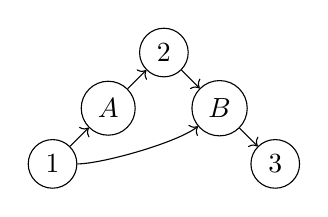
\begin{tikzpicture}[main/.style = {draw, circle}] 
        \node[main] (1) {$1$}; 
        \node[main] (A) [above right of=1] {$A$};
        \node[main] (2) [above right of=A] {$2$};
        \node[main] (B) [below right of=2] {$B$};
        \node[main] (3) [below right of=B] {$3$};
        \draw[->] (1) -- (A);
        \draw[->] (A) -- (2);
        \draw[->] (2) -- (B);
        \draw[->] (1) to [out=0,in=220,looseness=0.5](B);
        \draw[->] (B) -- (3);
        \end{tikzpicture}\caption{Graph}
        \end{subfigure}\hfill
        \begin{subfigure}{0.45\columnwidth}\centering
        \begin{tabular}{| m{2pt} || m{9pt} | m{9pt} ||} 
         \hline
         & A & B \\ [0.5ex] 
         \hline\hline
         1 & 1 & 1  \\ 
         \hline
         2 & -1 & 1 \\
         \hline
         3 & 0 & -1 \\
         \hline
         \hline
        \end{tabular}\caption{PFGAM}\end{subfigure}
        \caption{Computer-friendly version of Type I-IIA PFG.}\label{fig:I-IIA-cf}\end{minipage}
\end{figure} 

\subsection{Feasible PFGAM Set Creation}
The fundamental feature of this algorithm is that no previous knowledge on feasible PFGAMs is required by the user or the program itself. The user only needs to select the value of the variable \textbf{Bidi\_Ports}; 0 for TPC with EB, 1 for TPC with ESS and 2 for TPC with ESS and bidirectional output. Therefore, during the first step of the execution, each cell of the PFGAM takes all the possible values (column by column) to create all the possible combinations. Obviously, most of them cannot be implemented in the real world. Therefore, a set of rules is applied on the PFGAM to clear all the non-feasible matrices.
\subsubsection{Rule 1 (Port Bidirectionality)}
\begin{enumerate}[label=\Alph*)]
    \item The input (RES) port only produces power and therefore the power flow is unidirectional. Consequently, the elements of the first row (RES port) may have a value of 0 or 1. Additionally, the ESS or EB port both offers and receives power based on the current operation of TPC. Consequently, each cell in the second row can take any of the three values (-1, 0, 1). The output port can either be unidirectional where its cell value set is \{-1, 0\} or bidirectional where the value set is full. 
    \item Each bidirectional port must have at least one intake and one outtake of power. Equivalently:
    \begin{itemize}   
    \item The sum of the absolute values of all row elements of any bidirectional row must be greater than the absolute value of the sum of all row elements. 
    \end{itemize}
    \underline{Proof:} Sum(ABS) cannot be lesser than ABS(Sum). Supposing that Sum(ABS) is equal to ABS(Sum), the cell values of the port row have the same sign. Therefore, all connected SGs are either providing or consuming power from the port, which is not acceptable.
\end{enumerate}
\subsubsection{Rule 2 (SG I/O Existence)}
Similar to Rule 1B, each one of the nodes that represent an SG, must have at least one input and one output, therefore:
\begin{itemize}
    \item The sum of the absolute values (Sum(ABS)) of all column elements of each SG column must be greater than the absolute value of the sum (ABS(Sum)) of the same column elements. 
\end{itemize}

\subsubsection{Rule 3 (SG Interleaving Prohibition)} 
Some of the following rules, need to have information on the exact position (row, column) of each connection to its SG. To obtain a compressed version of this information, an n-digit numerical system can be used, where n is the number of all potential PFGAM cell values (3 in our case). Therefore, in this paper a ternary numerical system is used. Then, the declaration of the positions of LSB and MSB is performed. For column-wise encoding, the data is compressed column-wise and the LSB is the cell element of the first row. Therefore, a $3*SG$ PFGAM column-wise compression will produce an $1*SG$ matrix.

Specifically for Rule 3, interleaving of SGs is not permitted as this not constitutes a different power flow configuration. The researchers should decide later on the interleaving of the SGs based on the final converter topology and on power level.
\begin{itemize}
    \item The columns of a PFGAM should have a unique (different among each other) compressed column.
\end{itemize}
\subsubsection{Rule 4 (Use of Minimum Interconnections)}
The aim of both this study and the previous ones is to implement every power flow configuration with the minimum number of SGs and FCs, hence there has to be no overlap in the power flows. 
\begin{enumerate}[label=\Alph*)]\item To guarantee that, the algorithm follows the rule below, which was formulated by observing the resulting configurations of the previous works \cite{yang_synthesis_2015},\cite{zogogianni_non-isolated_2019},\cite{aljarajreh_synthesis_2021}.\\
The number of non-Type I SGs must be lower or equal to the maximum potentially required non-Type I SGs. This limit is based on the number of total SGs (h) and the number of Bidirectional Ports (Bidi\_Ports) and it is expressed as:
    \begin{small}
    \begin{equation}
    max\_non\_I[h]\end{equation}\end{small}
    where $max\_non\_I[h]$ is a list with the range limits:
    \begin{small}\begin{equation}max\_non\_I=[Min.SGs-Bidi\_Ports, Min.SGs]\end{equation}\end{small}
    and $Min.SGs$ is the minimum required number of SGs which is equal to two for all cases.
\item If two SGs have identical power flow paths, then this will be detected by Rule 3 and the PFGAM will be cleared out. However, a Type I SG in parallel with one branch of a Type II or III SG will not be filtered and therefore an additional rule is needed.
\begin{itemize}
    \item There shouldn't be a pair of any SGs, where any two cells in the same row are equal and non zero, provided that exactly one SG is Type I.
\end{itemize}\end{enumerate}

\subsubsection{Rule 5 (PFGAM Uniqueness)}
PFGAMs with the same configuration and interchanged names among the SGs are not considered unique. Therefore:
\begin{itemize}
    \item The compressed columns of a PFGAM should not be identical with any other PFGAM, even if the columns are interchanged in any way.
\end{itemize}

The first part of the algorithm is developed so that all feasible PFGAMs will be extracted. The algorithm is presented in a pseudocode form in Fig.\ref{fig:alg1} and explained below:
\begin{enumerate}
    \item \underline{Generate all possible PFGAMs}: For a given set of cell values \{-1,0,1\}, all possible PFGAMs can be generated by starting from a \( \mathbf{3 * N_{SG}} \) zero matrix X and systematically changing the value of each $x_{i,j}$ to produce all the combinations. The number of those combinations is $3^{3*N_{SG}}$, which means that it becomes huge even for small values of $N_{SG}$ ($N_{SG}=3\longrightarrow 19683$ combinations). This number can be significantly reduced by utilizing Rule 1A. Specifically, when creating the combinations for the first row (input port), the cell value $-1$ should not be included in the set of cell values, as the input port only produces power. Similar goes for the rest of the ports. By implementing those constraints the available combinations are reduced to $2^{2*N_{SG}}*3^{N_{SG}}$ ($N_{SG}=3\longrightarrow 192$ for the case of a single bidirectional port (ESS)).
    \item \underline{Algorithm Optimization}: The possible PFGAMs are generated column-by-column and the results are included in the set of PFGAMs so that they will be used during the generation of next column. When this happens, the initial results are obsolete (as they are included in the next results with the information of one more column included). Therefore they can be removed, prior to the column's rule check to reduce execution time.
    \item \underline{Rule Application to the PFGAMs}: Most of the suggested rules are applied, by definition, column-wise on the PFGAM. Therefore, the approach of PFGAM creation column-by-column has significant advantage as Rules 2, 3, 4, 5 are applied after the creation of each column, clearing out invalid PFGAMs prior to their full creation. On the contrary, Rule 1B is applied row-wise and consequently the complete PFGAM must be available.
\end{enumerate}
Following this procedure, all feasible PFGAMs are created and the next step of the method can be executed.\\
\RestyleAlgo{ruled}
\begin{figure}[!t]
 \removelatexerror
\begin{algorithm}[H]
%\caption{Feasible PFGAM Set Creation}\label{alg:one}
Initialize empty PFGAM set\;
Initialize $3\times SG$ PFGAM with zeros\; 
Insert it in the Set\;
\For{each column (\textbf{j}) of PFGAM}{
    \For{each row (\textbf{i}) of PFGAM}{
        \For{each available PFGAM(\textbf{l}) in PFGAM Set}{
            \For{each available cell value (\textbf{k})}{
                $PFGAM\_Set[l, i, j] \gets cell\_values[k]$\; }}}
    /*Column j has been created*/\;
    \underline{Remove} initial PFGAMs from Set\;
    \underline{Apply} Rules 2, 3, 4, 5\;    
    }/*All cells have been updated*/\;
    \underline{Apply} Rule 1B\;
    \underline{Find} the type of each SG\;
    \underline{Find} position of bidirectional SGs\;
\end{algorithm}\caption{Pseudocode for Feasible PFGAM Set Creation}\label{fig:alg1} \end{figure}

\begin{figure}[!t]
 \removelatexerror
\begin{algorithm}[H]
%\caption{Power Flow Configurations Creation}
%\label{alg:two}
$uni\_pool \gets unidirectional SGs$\;
$bidi\_pool \gets bididirectional SGs$\;
/*ports where a Bidi FC can be placed*/\;
$pool \gets [2, Bidi\_Ports+1]$\;
$inv\_pool \gets [1,3]-[1,3]\cap pool$\;
\eIf{no Type I SG exists}{
    \For{each port (\textbf{i}) of pool}{
        \For{each port (\textbf{j}) of inv\_pool}{
            $set \gets [set, i, j]$ /*assign ports(i, j) as FC placement pair*/\;} 
        \For{each port (\textbf{j}) of pool}{\If{1}{
            $set \gets [set, i, j]$ /*assign ports(i, j) as FC placement pair*/\;}}}
    }
    {$set \gets 2$\;
    \For{each non Type I bidirectional SG (j)}{
    \For{each port (i)}{\If{port i receives power}{$set \gets i$}}
    }
    }
    \For{each combination i of set}{
        {$configuration \gets zeros(column\_number(x)-length(bidi\_pool),column\_number(x)+3)$}\;
        \For{each element j of current combination i}{
            \For{each bidirectional SG k}{
                $y(j, bidi\_pool[k])\gets x(set[i, j], bidi\_pool[k])$\;
                $y(j, SG + set[i, j])\gets -x(set[i, j], bidi\_pool[k])$\;
            }}
        Store y in the power flow configurations set\;
    }
    %\eIf{uni\_pool empty}{Create uni\_port\;}
    %{$uni\_port \gets [1, 2, 3]$}
    $uni\_port \gets Create\_uni\_port()$\;
    \For{each unidirectional SG (j)}{
    \For{each port (i) in uni\_port connected to SG j}{
    \For{each PFG (k) with updated previous columns}{
                $y(length(bidi\_pool)/2+j,uni\_pool(j))\gets x(i,uni\_pool(j))$\;
                $y(length(bidi\_ind)/2+j,size(x,2)+i)\gets -x(i,uni\_pool(j))$\;
    }
    }
    }
\end{algorithm}\caption{Pseudocode for Power Flow Configurations Creation}\label{fig:alg2}\end{figure}
\subsection{FC Placement in PFGs}
For this step, the structure of the initial PFGAMs created in the previous section will be updated as shown in result Figs. \ref{fig:EB_summary}, \ref{fig:ESS_summary} and \ref{fig:ESS_Out_summary}. More specifically, three columns (one for each port) will be added right of the initial PFGAM. Additionally, below the initial PFGAM as many rows as the number of FCs needed will be added. This is necessary in order to correctly display the connections of different elements after the FC placement. Cells indicating connections between SGs and ports get zeroed now, if an FC is placed between the port and the SG. If a port both receives and offers power through the same bidirectional converter, a high value (10) is inserted in the corresponding cell, as there isn't any simple way to insert $\pm1$ in an array. This part of the algorithm is presented in a pseudocode form in Fig. \ref{fig:alg2} and is described below. 
\subsubsection{Determination of FC positions}
First of all, the SGs are separated in two different data pools (uni-pool and bidi-pool), based on their suitability for unidirectional or bidirectional FC placement. By definition, one SG cannot be bidirectional. Therefore, for a bidirectional FC to be utilized, two fitting SGs must be combined. By SG fitness it is meant that two SGs must have exactly two power flow vectors that are complementary, i.e. they exhibit opposite power flow. To search up for these SGs, the procedure below can be followed:
\begin{enumerate}[label=\alph*)]
    \item For the case of TPC with EB, no bidirectional FC will be used and therefore this procedure is bypassed.
    \item All possible combinations of SG pairs are created.
    \item For the rest of the cases, a 2*2 array is created for each SG pairs. The first row of the array elements consist of the corresponding elements (same SGs) of the ESS row of the PFGAM, while the second row consists of:
    \begin{itemize}
        \item \underline{Bidirectional Output}: the corresponding elements of the output row of the PFGAM.
        \item \underline{Unidirectional Output}: the first row multiplied by -1.
    \end{itemize}
    Cascaded configuration Type I-I is excluded from the process, as in this case, even though there is a bidirectional port, no bidirectional FC is used. 
    \item The sums of the primary and secondary diagonal of the array are calculated.
    \item If those sums are opposite to each other and the absolute sum of each is greater than one, then this SG pair may be interfaced with a bidirectional FC. This is because that condition guarantees that both rows offer and receive power complementary to both SGs and themselves, which means that a bidirectional power path is existent.
\end{enumerate}

Furthermore, the range of ports where a bidirectional FC can be placed is determined from the range below:
\begin{small}
    \begin{equation}
    Bidi\_FC\_Ports\_pool = [2, Bidi\_Ports+1]
    \label{eq:pool}\end{equation}
\end{small}
This equation summarizes that in case of TPC with EB, no bidirectional FC is placed, while in case of a TPC with ESS either port 2 (Unidirectional output) or ports 2 and 3 (Bidirectional output) can be interfaced with a bidirectional FC. The complementary set (inv\_Bidi\_FC\_Ports\_pool) is also created, as it is used for the creation of ports pairs where FCs will be placed.
\subsubsection{Bidirectional FC Placement}
Diving into the potential placement of bidirectional FCs, the algorithm checks if a Type I SG is existent in the PFG. \textbf{If not}, no SISO converter will be used, as each FC will either be bidirectional or will be used for the joint connection of a port to two SGs as shown in Fig. 7 of \cite{aljarajreh_synthesis_2021}. In this case, it is crucial to determine in which ports will the FCs be connected to. Depending on the number of required FCs, connection pairs are created both between the Bidi\_FC\_Ports\_pool and the inv\_Bidi\_FC\_Ports\_pool elements, but also between the Bidi\_FC\_Ports\_pool elements themselves. Then, for each created combination set, a bidirectional FC is placed into each port of the set. The FCs are placed in between the bidirectional SGs (bidi\_pool). \textbf{Alternatively}, SISO converters will be used and the only bidirectional FC will be connected between SGs contained in bidi\_pool and the first port (by convention) of Bidi\_FC\_Ports\_pool. 
\subsubsection{Unidirectional FC placement}
At this point, the placement of the bidirectional FCs is finished. Now, one unidirectional FC needs to be placed in each unidirectional SG to achieve full controllability of the system. The Create\_uni\_port function is called, having the following functionality; if uni\_pool is empty but a Type I SG is existent, that means that there are only two SGs. Apparently, a unidirectional FC should not be placed on the port that has the bidirectional power flow, so a list called uni\_port is created with the rest of the ports where a unidirectional FC is acceptable. The FC can be placed between any port of uni\_port that is connected to this SG and the point X\{A, B, etc.\} of intersection of power flow vectors. If the SG is Type-I, there is no need to put FCs in all ports, as there are only two ports involved and placing the FC in one port is identical to placing the FC in the other port. Similar to the initial PFGAM creation, the extended PFGAM is updated column-by-column (SG-by-SG).

\begin{figure*}[!t]

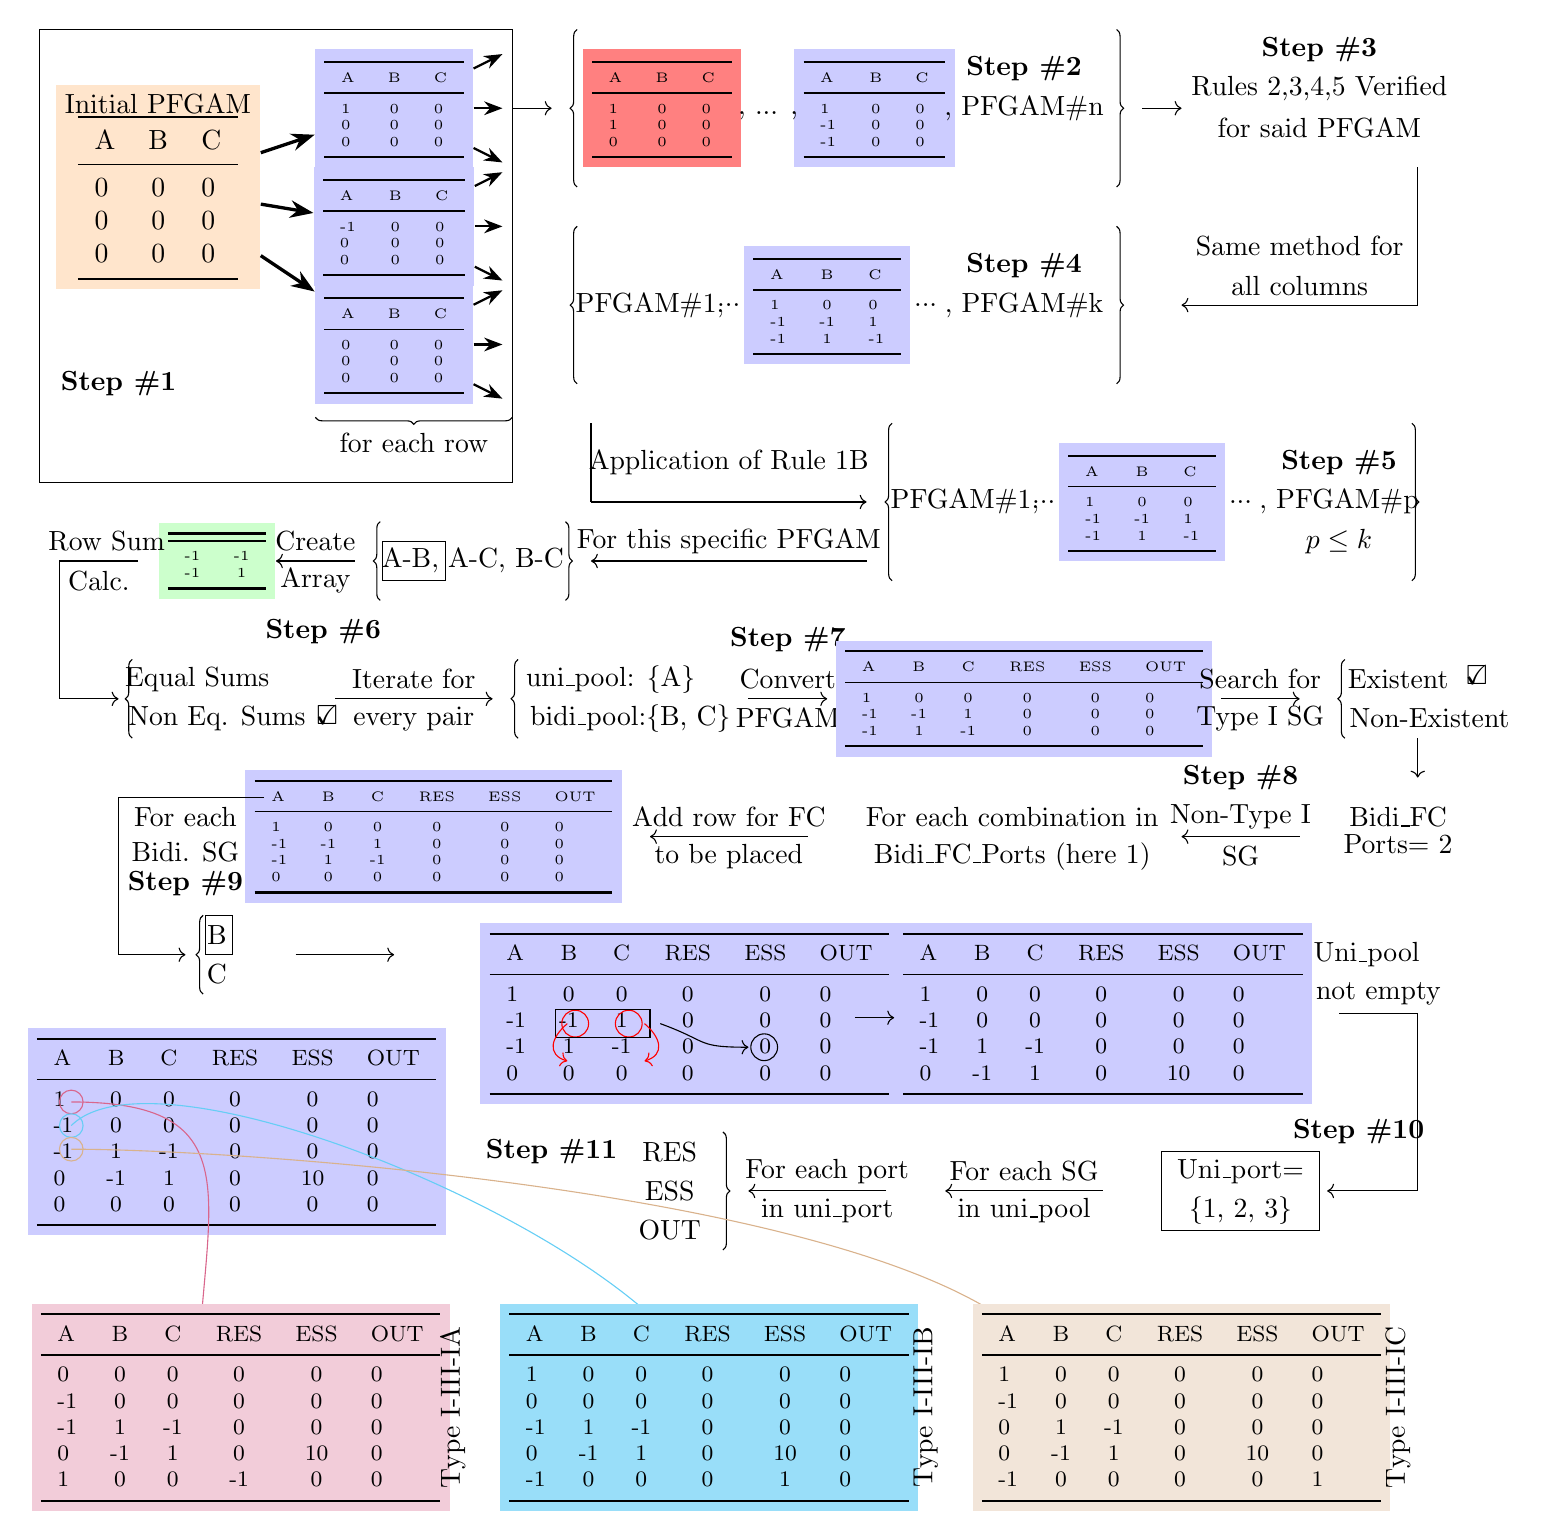
\begin{tikzpicture}[]
\draw (-1.5,0) rectangle (4.5,-5.75);
    \node [shape=rectangle,fill=orange!20, align=center](table1) at (0.0,-2.0) {
            Initial PFGAM \\
            \begin{tabular}{lcl} \toprule
                A & B & C  \\ \midrule
                0 & 0 & 0 \\
                0 & 0 & 0 \\
                0 & 0 & 0\\
                \bottomrule
            \end{tabular}
        };
    \node [shape=rectangle,fill=blue!20, align=center](table2) at (3.0,-1.0) {
            \\
            \tiny
            \begin{tabular}{lcl} \toprule
                A & B & C  \\ \midrule
                1 & 0 & 0 \\
                0 & 0 & 0 \\
                0 & 0 & 0\\
                \bottomrule
            \end{tabular}
        };
    \node [shape=rectangle,fill=blue!20, align=center](table3) at (3.0,-2.5) {
            \\
            \tiny
            \begin{tabular}{lcl} \toprule
                A & B & C  \\ \midrule
                -1 & 0 & 0 \\
                0 & 0 & 0 \\
                0 & 0 & 0\\
                \bottomrule
            \end{tabular}
        };    
    \node [shape=rectangle,fill=blue!20, align=center](table4) at (3.0,-4.0) {
            \\
            \tiny
            \begin{tabular}{lcl} \toprule
                A & B & C  \\ \midrule
                0 & 0 & 0 \\
                0 & 0 & 0 \\
                0 & 0 & 0\\
                \bottomrule
            \end{tabular}
        };       
    \node [] (arrow1) at (4.5,-0.25){}; \node [] (arrow2) at (4.5,-1.0){}; \node [] (arrow3) at (4.5,-1.75){};
    \node [] (arrow4) at (4.5,-1.75){}; \node [] (arrow5) at (4.5,-2.5){}; \node [] (arrow6) at (4.5,-3.25){};
    \node [] (arrow7) at (4.5,-3.25){}; \node [] (arrow8) at (4.5,-4.0){}; \node [] (arrow9) at (4.5,-4.75){};
    \draw [very thick, -Stealth] (table1) -- (table2);
    \draw [very thick, -Stealth] (table1) -- (table3);
    \draw [very thick, -Stealth] (table1) -- (table4);
    \node at (-0.5,-4.5) {\textbf{Step \#1}}; 
    \draw [thick, -Stealth] (table2) -- (arrow1); \draw [thick, -Stealth] (table2) -- (arrow2); \draw [thick, -Stealth] (table2) -- (arrow3);
    \draw [thick, -Stealth] (table3) -- (arrow4); \draw [thick, -Stealth] (table3) -- (arrow5); \draw [thick, -Stealth] (table3) -- (arrow6);
    \draw [thick, -Stealth] (table4) -- (arrow7); \draw [thick, -Stealth] (table4) -- (arrow8); \draw [thick, -Stealth] (table4) -- (arrow9);
    \draw[decoration={brace,mirror, raise=5pt},decorate](2,-4.75) -- node[right=6pt] {} (4.5,-4.75);
    \node at (3.25,-5.25) {for each row};
    \draw[->] (4.5,-1) -- (5.0,-1);
    \draw[decoration={brace,mirror,raise=5pt},decorate](5.5,0) -- node[right=6pt] {} (5.5,-2);
    \draw[decoration={brace,raise=5pt},decorate](12,0) -- node[right=6pt] {} (12,-2);
        \node [shape=rectangle,fill=red!50, align=center](table3) at (6.4,-1) {
            \\
            \tiny
            \begin{tabular}{lcl} \toprule
                A & B & C  \\ \midrule
                1 & 0 & 0 \\
                1 & 0 & 0 \\
                0 & 0 & 0\\
                \bottomrule
            \end{tabular}
        };  
    %\node at (7.5,-1) {,};    
    \node [shape=rectangle,fill=blue!20, align=center](table3) at (9.1,-1) {
            \\
            \tiny
            \begin{tabular}{lcl} \toprule
                A & B & C  \\ \midrule
                1 & 0 & 0 \\
                -1 & 0 & 0 \\
                -1 & 0 & 0\\
                \bottomrule
            \end{tabular}
        };    
    %\node at (6.25,-1) {PFGAM\#1,};  \node at (7.25,-1) {...}; 
    \node at (7.75,-1.1) {, ... ,};\node at (11,-1) {, PFGAM\#n}; 
    \node at (11,-0.5) {\textbf{Step \#2}}; 
    \draw[->] (12.5,-1) -- (13,-1);
    \node at (14.75,-0.25) {\textbf{Step \#3}}; 
    \node at (14.75,-0.75) {Rules 2,3,4,5 Verified};
    \node at (14.75,-1.25) {for said PFGAM};
    \draw[] (16,-1.75) -- (16,-3.5);\draw[->] (16,-3.5) -- (13,-3.5);
    \node at (14.5,-2.75) {Same method for}; 
    \node at (14.5,-3.25) {all columns}; 
    \node at (6.25,-3.5) {PFGAM\#1,};  \node at (7.25,-3.5) {...}; \node at (9.75,-3.5) {...};\node at (11,-3.5) {, PFGAM\#k};
    %\node at (11,-4) {$k\le n$}; 
    \node at (11,-3) {\textbf{Step \#4}}; 
    \draw[decoration={brace,mirror,raise=5pt},decorate](5.5,-2.5) -- node[right=6pt] {} (5.5,-4.5);
    \draw[decoration={brace,raise=5pt},decorate](12,-2.5) -- node[right=6pt] {} (12,-4.5);
        \node [shape=rectangle,fill=blue!20, align=center](table3) at (8.5,-3.5) {
            \\
            \tiny
            \begin{tabular}{lcl} \toprule
                A & B & C  \\ \midrule
                1 & 0 & 0 \\
                -1 & -1 & 1 \\
                -1 & 1 & -1\\
                \bottomrule
            \end{tabular}        
        };    
    \draw[] (5.5,-5) -- (5.5,-6);\draw[->] (5.5,-6) -- (9,-6);
    \node at (10.25,-6) {PFGAM\#1,};  \node at (11.25,-6) {...}; \node at (13.75,-6) {...};\node at (15,-6) {, PFGAM\#p}; \node at (15,-6.5) {$p\le k$}; 
    \node at (15,-5.5) {\textbf{Step \#5}}; 
    \draw[decoration={brace,mirror,raise=5pt},decorate](9.5,-5) -- node[right=6pt] {} (9.5,-7);
    \draw[decoration={brace,raise=5pt},decorate](15.75,-5) -- node[right=6pt] {} (15.75,-7);
        \node [shape=rectangle,fill=blue!20, align=center](table3) at (12.5,-6) {
            \\
            \tiny
            \begin{tabular}{lcl} \toprule
                A & B & C  \\ \midrule
                1 & 0 & 0 \\
                -1 & -1 & 1 \\
                -1 & 1 & -1\\
                \bottomrule
            \end{tabular}};
    \node at (7.25,-5.5) {Application of Rule 1B}; 
     \draw[->] (9,-6.75) -- (5.5,-6.75);
     \node at (7.25,-6.5) {For this specific PFGAM};
     \draw[decoration={brace,raise=5pt},decorate](5,-6.25) -- node[right=6pt] {} (5,-7.25);
     \draw[decoration={brace, mirror, raise=5pt},decorate](3,-6.25) -- node[right=6pt] {} (3,-7.25);
    \node at (4,-6.75) {A-B, A-C, B-C};
    \draw (2.85,-6.5) rectangle (3.65,-7);
    \draw[->] (2.5,-6.75) -- (1.5,-6.75);
    \node at (2,-6.5) {Create};
    \node at (2,-7) {Array};
    \node at (2.1,-7.65) {\textbf{Step \#6}};
        \node [shape=rectangle,fill=green!20, align=center](mat) at (0.75,-6.75) {
            \tiny
            \begin{tabular}{lc} \toprule
                 \midrule
                -1 & -1 \\
                -1 & 1  \\
                \bottomrule
            \end{tabular}};
    \node at (-0.65,-6.5) {Row Sum};
    \node at (-0.75,-7) {Calc.};
    \draw[] (-0.25,-6.75) -- (-1.25,-6.75);\draw[] (-1.25,-6.75) -- (-1.25,-8.5);\draw[->] (-1.25,-8.5) -- (-0.5,-8.5);
    \draw[decoration={brace,mirror,raise=5pt},decorate](-0.15,-8) -- node[right=6pt] {} (-0.15,-9);
    \node at (0.5,-8.25) {Equal Sums};
    \node at (0.75,-8.75) {Non Eq. Sums};
    \node at (2.15,-8.7) {\mbox{\ooalign{$\checkmark$\cr\hidewidth$\square$\hidewidth\cr}}};
     \draw[->] (2.25,-8.5) -- (4.25,-8.5);
    \node at (3.25,-8.25) {Iterate for};
    \node at (3.25,-8.75) {every pair};
     \draw[decoration={brace,mirror,raise=5pt},decorate](4.75,-8) -- node[right=6pt] {} (4.75,-9);
     \node at (5.75,-8.25) {uni\_pool: \{A\}};\node at (6,-8.75) {bidi\_pool:\{B, C\}};
     \draw[->] (7.5,-8.5) -- (8.5,-8.5); \node at (8,-8.25) {Convert};\node at (8,-8.75) {PFGAM};\node at (8,-7.75) {\textbf{Step \#7}};
        \node [shape=rectangle,fill=blue!20, align=center](mat2) at (11,-8.5) {
            \tiny
            \begin{tabular}{lccccl} \toprule
                A & B & C &RES &ESS &OUT \\ \midrule
                1 & 0 & 0& 0& 0& 0 \\
                -1 & -1 & 1& 0& 0& 0 \\
                -1 & 1 & -1& 0& 0& 0\\
                \bottomrule
            \end{tabular}};   
    \draw[decoration={brace,mirror,raise=5pt},decorate](15.25,-8) -- node[right=6pt] {} (15.25,-9);    
    \node at (15.75,-8.25) {Existent};
    \node at (16.15,-8.75) {Non-Existent};
    \node at (16.75,-8.2) {\mbox{\ooalign{$\checkmark$\cr\hidewidth$\square$\hidewidth\cr}}};
     \draw[->] (13.5,-8.5) -- (14.5,-8.5);
    \node at (14,-8.25) {Search for};
    \node at (14,-8.75) {Type I SG};
    \draw[->] (16,-9) -- (16,-9.5);
    \node at (15.75,-10.0) {Bidi\_FC};
    \node at (15.75,-10.35) {Ports= 2};
    \draw[->] (14.5,-10.25) -- (13,-10.25);
    %\node at (12.75,-109.75) {No Bidirectional};
    \node at (13.75,-9.5) {\textbf{Step \#8}};
    \node at (13.75,-10.0) {Non-Type I};
    \node at (13.75,-10.5) {SG};
    \node at (10.85,-10) {For each combination in};
    \node at (10.85,-10.5) {Bidi\_FC\_Ports (here 1)};
    \draw[->] (8.25,-10.25) -- (6.25,-10.25);
    \node at (7.25,-10) {Add row for FC};
    \node at (7.25,-10.5) {to be placed};
        \node [shape=rectangle,fill=blue!20, align=center](mat3) at (3.5,-10.25) {
            \tiny
            \begin{tabular}{lccccl} \toprule
                A & B & C &RES &ESS &OUT \\ \midrule
                1 & 0 & 0& 0& 0& 0 \\
                -1 & -1 & 1& 0& 0& 0 \\
                -1 & 1 & -1& 0& 0& 0\\
                0 & 0 & 0& 0& 0& 0\\
                \bottomrule
            \end{tabular}};  
    \node at (0.35,-10) {For each};
    \node at (0.35,-10.45) {Bidi. SG};
    \node at (0.35,-10.85) {\textbf{Step \#9}};
    \draw[decoration={brace,mirror,raise=5pt},decorate](0.75,-11.25) -- node[right=6pt] {} (0.75,-12.25); 
    \draw[] (1.35,-9.75) -- (-0.5,-9.75);\draw[] (-0.5,-9.75) -- (-0.5,-11.75);\draw[->] (-0.5,-11.75) -- (0.35,-11.75);
    \node at (0.75,-11.5) {B}; \draw (0.6,-11.25) rectangle (0.95,-11.75);\draw[->] (1.75,-11.75) -- (3,-11.75);
    \node at (0.75,-12.0) {C};
    \node [shape=rectangle,fill=blue!20, align=center](mat4) at (6.75,-12.50) {
            \footnotesize
            \begin{tabular}{lccccl} \toprule
                A & B & C &RES &ESS &OUT \\ \midrule
                1 & 0 & 0& 0& 0& 0 \\
                -1 & -1 & 1& 0& 0& 0 \\
                -1 & 1 & -1& 0& 0& 0\\
                0 & 0 & 0& 0& 0& 0\\
                \bottomrule
            \end{tabular}}; 
    \draw[red] (5.3,-12.625) circle (0.17); 
    \draw[red] (5.98,-12.625) circle (0.17); 
    \draw (7.7,-12.925) circle (0.17);
    \draw (5.05,-12.45) rectangle (6.25,-12.8);
    \draw[->,red] (5.2,-12.625) to [out=220,in=165,looseness=1.5] (5.2,-13.1);
    \draw[->,red] (6.18,-12.625) to [out=320,in=15,looseness=1.5] (6.18,-13.1);
    \draw[->] (6.38,-12.625) to [out=340,in=180,looseness=1.5] (7.5,-12.925);   
    
    \node [shape=rectangle,fill=blue!20, align=center](mat4) at (12,-12.5) {
            \footnotesize
            \begin{tabular}{lccccl} \toprule
                A & B & C &RES &ESS &OUT \\ \midrule
                1 & 0 & 0& 0& 0& 0 \\
                -1 & 0 & 0& 0& 0& 0 \\
                -1 & 1 & -1& 0& 0& 0\\
                0 & -1 & 1& 0& 10& 0\\
                \bottomrule
            \end{tabular}};     
    %\node at (7,-10.25) {For each element in current combination(1 in this case)};
    \draw[->] (8.85,-12.55) -- (9.35,-12.55);
    \draw[] (15.0,-12.5) -- (16.0,-12.5);
    \draw[] (16.0,-12.5) -- (16.0,-14.75);
    \draw[->] (16.0,-14.75) -- (14.85,-14.75);
    \node at (15.35,-11.75) {Uni\_pool};
    \node at (15.5,-12.25) {not empty};
    \node at (15.25,-14.0) {\textbf{Step \#10}};
    \draw (12.75,-14.25) rectangle (14.75,-15.25);
    \node at (13.75,-14.5) {Uni\_port=};
    \node at (13.75,-15.0) {\{1, 2, 3\}};
    \draw[->] (12.0,-14.75) -- (10,-14.75);
    \node at (11,-14.5) {For each SG};
    \node at (11,-15.0) {in uni\_pool};
    \draw[->] (9.25,-14.75) -- (7.5,-14.75);
    \node at (8.5,-14.5) {For each port};
    \node at (8.5,-15.0) {in uni\_port};
    \draw[decoration={brace,raise=5pt},decorate](7,-14.0) -- node[right=6pt] {} (7,-15.5);
    \node at (5.0,-14.25) {\textbf{Step \#11}};
    \node at (6.5,-14.25) {RES};
    \node at (6.5,-14.75) {ESS};
    \node at (6.5,-15.25) {OUT};
    \node [shape=rectangle,fill=blue!20, align=center](mat4) at (1,-14.00) {
            \footnotesize
            \begin{tabular}{lccccl} \toprule
                A & B & C &RES &ESS &OUT \\ \midrule
                1 & 0 & 0& 0& 0& 0 \\
                -1 & 0 & 0& 0& 0& 0 \\
                -1 & 1 & -1& 0& 0& 0\\
                0 & -1 & 1& 0& 10& 0\\
                 0 &0 & 0& 0& 0& 0\\
                \bottomrule
            \end{tabular}};   
    \draw[purple!60] (-1.1,-13.62) circle (0.15);
    \draw[->,purple!60] (-1.1,-13.62) to [out=0,in=90,looseness=1.5] (0.5,-17.50);
    \draw[cyan!60] (-1.1,-13.92) circle (0.15);
    \draw[->,cyan!60] (-1.1,-13.92) to [out=45,in=90,looseness=0.5] (7.0,-17.50);
    \draw[brown!60] (-1.1,-14.22) circle (0.15);
    \draw[->,brown!60] (-1.1,-14.22) to [out=0,in=90,looseness=0.5] (11.5,-17.50);
    \node [shape=rectangle,fill=purple!20, align=center](mat4) at (1.05,-17.50) {
            \footnotesize
            \begin{tabular}{lccccl} \toprule
                A & B & C &RES &ESS &OUT \\ \midrule
                0 & 0 & 0& 0& 0& 0 \\
                -1 & 0 & 0& 0& 0& 0 \\
                -1 & 1 & -1& 0& 0& 0\\
                0 & -1 & 1& 0& 10& 0\\
                 1 &0 & 0& -1& 0& 0\\
                \bottomrule
            \end{tabular}}; 
    \node [rotate=90] at (3.75,-17.5) {Type I-III-IA};
    \node [shape=rectangle,fill=cyan!40, align=center](mat4) at (7.0,-17.50) {
            \footnotesize
            \begin{tabular}{lccccl} \toprule
                A & B & C &RES &ESS &OUT \\ \midrule
                1 & 0 & 0& 0& 0& 0 \\
                0 & 0 & 0& 0& 0& 0 \\
                -1 & 1 & -1& 0& 0& 0\\
                0 & -1 & 1& 0& 10& 0\\
                 -1 &0 & 0& 0& 1& 0\\
                \bottomrule
            \end{tabular}}; 
    \node [rotate=90] at (9.75,-17.5) {Type I-III-IB};
    \node [shape=rectangle,fill=brown!20, align=center](mat4) at (13.0,-17.50) {
            \footnotesize
            \begin{tabular}{lccccl} \toprule
                A & B & C &RES &ESS &OUT \\ \midrule
                1 & 0 & 0& 0& 0& 0 \\
                -1 & 0 & 0& 0& 0& 0 \\
                0 & 1 & -1& 0& 0& 0\\
                0 & -1 & 1& 0& 10& 0\\
                 -1 &0 & 0& 0& 0& 1\\
                \bottomrule
            \end{tabular}}; 
    \node [rotate=90] at (15.75,-17.5) {Type I-III-IC};
\end{tikzpicture}
\caption{Abstract display of the algorithm's execution, focused on Type I-III-I PFG.}
\label{fig:case}
\end{figure*}

\section{Case Study}
To further clarify the procedure described above, a case study will be performed in this section, where a PFG will be extracted. For the sake of completeness, a PFG with two bidirectional ports ($Bidi\_Ports=2$) will be examined so that every part of the algorithm is described. The PFG examined is \textbf{Type I-III-I}, which will lead to the power flow configurations I-III-IA, I-III-IB and I-III-IC. The algorithm execution for this case study is depicted in Fig. \ref{fig:case}, where different steps are denoted with \textbf{Step \#} and arrows indicate the serial execution of the algorithm.

This PFG will be derived from the first part of the algorithm. Initially, based on the $Bidi\_Ports$ parameter, the number of the required SGs is computed. For $Bidi\_Ports=2$, SGs may be between 2 and 4. Starting with 2, all feasible PFGs are derived. Similarly, for $SG=3$, a $3*3$ matrix is created and filled with zeros. Now, for the first column, one value of the set \{1,-1,0\} is inserted in the cell of the first row. The altered PFGAM (with only one cell different) is stored in the set of potential PFGAMs, without deleting the initial $3*3$ zero PFGAM used for its creation. This is repeated for the remaining values of the set (\textbf{Step \#1}). The procedure is then performed for the cell of the second row (while still being in column 1), with the difference that now there isn't only one PFGAM where the cell value must be changed, but the operation must be done for all PFGAM instances (zero PFGAM, plus 3 cases created for the previous cell). It becomes apparent that the possible PFGAMs increase in number in each iteration. By carrying on this procedure, all combinations of first column values are stored in different PFGAMs (\textbf{Step \#2}). One of these cases is the one that we are interested to, which is displayed in Fig. \ref{fig:case} in its current form. As it was stated in the previous section, a PFGAM set number reduction is performed after each column, by removing the initial PFGAMs that were used to update the set. For the first row, only the initial full zero PFGAM must be deleted. For graph simplicity, this procedure is not depicted in the relevant figure.

Prior to moving on the second column (SG), the rule application for the rules that are applied column-wise must be performed, to clear every non-feasible PFG (\textbf{Step \#3}). By simple observation it can be seen that the Type I-III-I PFGAM complies with Rules 2, 3, 4, 5. On the contrary, for reference purposes, the PFGAM displayed in Fig. must be deleted as it violates Rule 2. After rule application, the same procedure is followed for the rest of the columns (\textbf{Step \#4}). Then, the complete PFGAMs are formed and the last Rule 1B must be checked (row-wise). Again, the PFGAM of interest is compliant (\textbf{Step \#5}).

Moving to the second part of the algorithm, the suitable FCs must be placed in each PFGs. The first step is to separate the SGs suitable for unidirectional and bidirectional FC placement in two different pools ($uni\_pool$ and $bidi\_pool$, \textbf{Step \#6}). The possible combinations of SG pairs are created (A-B, A-C, B-C). For the first pair (A-B) the array created is shown. The sum of the primary diagonal is \textbf{0}, while the one of the secondary is \textbf{-2}.  The two sums are not equal, meaning that the two SGs  cannot form a pair for a bidirectional FC placement. The same method is followed for the rest of the SG pairs leading to $uni\_pool=\{A\}$ and $bidi\_pool=\{B, C\}$. According to Eq. \ref{eq:pool}, in our case, the bidirectional FC can be placed in the power path of either the ESS or the output port.

Having separated the bidirectional and unidirectional SGs, the FC placement starts with the bidirectional one. To store the additional information of how the FCs are connected to the PFGs, one additional column for each port and one extra row for each FC is added to the PFGAM (\textbf{Step \#7}). The row will be added one at a time, as the algorithm decides during the execution the number of FCs required for each PFG. To determine in which ports will the FC be placed, the following procedure is followed (\textbf{Step \#8}). Checking whether the PFGAM contains any Type I SG, two are found. Therefore, one bidirectional FC will be placed between the two bidirectional SGs. For contractual reasons, it is selected that the FC is placed on the port that is first encountered by the algorithm (here ESS port). Prior FC placement, a row is added to the PFGAM. For each bidirectional SG, the FC is inserted between the SG and the corresponding port, leading to the zeroing of the relevant cells and the transfer of their original values in the row of the FC (\textbf{Step \#9}), as shown in Fig. \ref{fig:case}. 

Then, one unidirectional FC will be placed in each unidirectional SG. The $Create\_uni\_port()$ function is called, but the PFGAM of interest does not belong to the special cases addressed by the function, so $uni\_ports={1, 2, 3}$ (\textbf{Step \#10}). For the first and only unidirectional SG (A), an FC is placed in one port of the $uni\_port$ each time, creating three different cases; Type I-III-IA, I-III-IB and I-III-IC (\textbf{Step \#11}).

\section{Results}
Based on the developed algorithm, all possible PFG configurations can be extracted for three different system options, namely the TPC with EB, and TPC with ESS and unidirectional/bidirectional output. The configurations are discussed in the following subsections, where indicative results are shown. To further increase ease of use of the algorithm, a graphical user interface was developed in MATLAB. Via this app, the user can choose between finding the PFGs with or without the corresponding FCs, for the required system characteristics. The results are displayed one at a time both in their PFGAM and their graph forms. In Fig. \ref{fig:app}, the app is shown presenting the resulting PFG of type I-III-IA, which was examined in the case study.

\textbf{All results} can be found in the relevant \textbf{\href{https://github.com/gsalagiannis/Algorithmic-approach-on-the-exctraction-of-power-flow-configurations-for-R2P2-DC-DC-converters}{Github repository}}. The \textbf{execution time} has an order of magnitude of \textbf{1s}.

\begin{figure}[htbp]
    \centering
    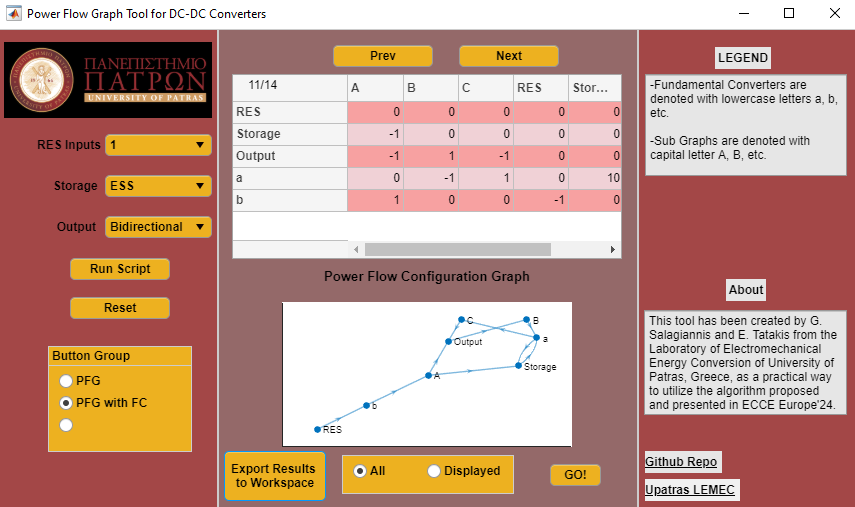
\includegraphics[width=0.5\textwidth]{App.png} % Replace 'your_figure_file' with the filename of your figure
    \caption{The developed tool in MATLAB.}
    \label{fig:app}
\end{figure}

%\subsection{PFG configurations for TPS with EB}
For the design of TPCs with EB, only unidirectional FCs are required. Furthermore, no control is required for the power flow of the EB, leading to a direct (without the interference of a converter) connection between that and parts of the rest of the system. The full set of available configurations have been initially grouped and studied by \cite{zogogianni_non-isolated_2019}. In this paper, all those PFGs were generated by the proposed algorithm, with one configuration presented in Fig. \ref{fig:EB_summary}. In this Figure, both the PFGAM and the corresponding graph are shown. The gray coloured cells do not have any essential meaning, as two ports cannot exchange power directly. The red coloured cells indicate the connections on the initial PFGAM that need to be deleted (zero inserted) after the FC placement.

\begin{figure}[htbp]\centering
        
        \begin{subfigure}{0.45\columnwidth}\centering
        {\footnotesize\begin{tabular}{| m{2pt} || m{7pt} | m{7pt}| m{7pt} | m{7pt} | m{7pt}  ||} 
         \hline
         & A & B & 1 & 2 & 3  \\ [0.5ex] 
         \hline\hline
         1 & 1 & \cellcolor{red!30}1 &  \cellcolor{gray!30} &  \cellcolor{gray!30} &  \cellcolor{gray!30} \\ 
         \hline
         2 & \cellcolor{red!30}-1 & 1 & \cellcolor{gray!30} &  \cellcolor{gray!30} &  \cellcolor{gray!30}\\
         \hline
         3 & -1 & -1 & \cellcolor{gray!30} &  \cellcolor{gray!30} &  \cellcolor{gray!30}\\
         \hline
         a & -1 & 0 & 0 & 1 & 0\\
         \hline
         b & 0 & 1 & -1 & 0 & 0\\
      \hline\hline
        \end{tabular}}\caption{Type IIA-III PFGAM}\end{subfigure}
        \begin{subfigure}{0.45\columnwidth}\centering
         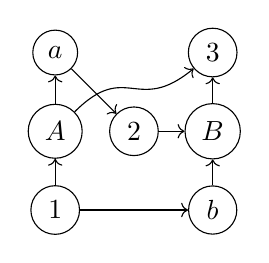
\begin{tikzpicture}[main/.style = {draw, circle}] 
         \node[main] at (0, 0) (1) {$1$}; 
        \node[main] at (0, 1) (A) {$A$};
        \node[main] at (0, 2) (a) {$a$};
        \node[main] at (1, 1) (2) {$2$};
        \node[main] at (2, 0) (b) {$b$};
        \node[main] at (2, 1) (B) {$B$};
        \node[main] at (2, 2) (3) {$3$};
        \draw[->] (1) -- (A);
        \draw[->] (A) -- (a);
        \draw[->] (A) to [out=45,in=220,looseness=1.5] (3);
        \draw[->] (a) -- (2);
        \draw[->] (1) -- (b);
        \draw[->] (b) -- (B);
        \draw[->] (2) -- (B);
        \draw[->] (B) -- (3);
        \end{tikzpicture}\caption{Type IIA-III Graph}
        \end{subfigure}\hfill
        \caption{Possible configuration of TPC with EB}\label{fig:EB_summary}
\end{figure} 

%\subsection{PFG configurations for TPC with ESS}
For ESS integration, a bidirectional FC needs to be placed between the ESS port and the rest of the system, with the exception of the Type I-I PFG. Some available configurations have been initially grouped and studied by \cite{yang_synthesis_2015}. Notably, only PFGs with at least one Type I SG were presented. On the contrary, in this paper, all feasible PFGs were generated by the proposed algorithm, with some results shown in Fig. \ref{fig:ESS_summary}.

\begin{figure}    
        \begin{subfigure}{0.45\columnwidth}\centering
        {\footnotesize\begin{tabular}{| m{2pt} || m{7pt} | m{7pt}| m{7pt} | m{7pt} | m{7pt}  ||} 
         \hline
         & A & B & 1 & 2 & 3 \\ [0.5ex] 
         \hline\hline
         1 & \cellcolor{red!30}1 & \cellcolor{red!30}1 &  \cellcolor{gray!30} &  \cellcolor{gray!30} &  \cellcolor{gray!30} \\ 
         \hline
         2 & \cellcolor{red!30}-1 &\cellcolor{red!30} 1 & \cellcolor{gray!30} &  \cellcolor{gray!30} &  \cellcolor{gray!30}\\
         \hline
         3 & -1 & -1 & \cellcolor{gray!30} &  \cellcolor{gray!30} &  \cellcolor{gray!30}\\
         \hline
         a & -1 & 1 & 0 & \cellcolor{cyan!30}10 & 0\\
         \hline
         b & 1 & 1 & -1 & 0 & 0\\
      \hline\hline
        \end{tabular}}\caption{Type II-IIIA PFGAM}\end{subfigure}
        \begin{subfigure}{0.65\columnwidth}\centering
         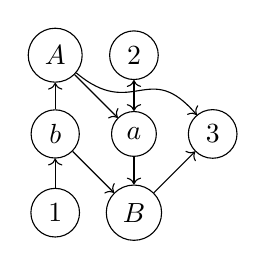
\begin{tikzpicture}[main/.style = {draw, circle}] 
        \node[main] at (0, 0) (1) {$1$}; 
        \node[main] at (1, 1) (a) {$a$};
        \node[main] at (1, 2) (2) {$2$};
        \node[main] at (1, 0) (B) {$B$};
        \node[main] at (0, 2) (A) {$A$};
        \node[main] at (0, 1) (b) {$b$};
        \node[main] at (2, 1) (3) {$3$};
        \draw[->] (1) -- (b);
        \draw[<->] (2) -- (a);
        \draw[->] (b) -- (A);
        \draw[->] (b) -- (B);
        \draw[->] (a) -- (B);
        \draw[->] (A) -- (a);
        \draw[->] (A) to [out=320,in=130,looseness=1.5] (3);
        \draw[->] (B) -- (3);
        \end{tikzpicture}\caption{Type II-IIIA Graph}
        \end{subfigure}\hfill
        \caption{Possible configuration of TPC with ESS}\label{fig:ESS_summary}
\end{figure} 
%\subsection{PFG configurations for TPC with ESS and bidirectional Output}
To incorporate both an ESS and a bidirectional output, a bidirectional power path needs to be established between the two ports. This can be achieved either with one or two bidirectional FCs, depending on the PFG configuration. The full set of available configurations have been initially grouped and studied by \cite{aljarajreh_synthesis_2021}, with the exception of PFGs I-IIA and I-IIB. In this paper, all PFGs were generated by the proposed algorithm, with some results presented in Fig. \ref{fig:ESS_Out_summary}.
\begin{figure}
       \begin{subfigure}{0.45\columnwidth}\centering
        {\footnotesize\begin{tabular}{| m{2pt} || m{7pt}| m{7pt}| m{7pt}| m{7pt} | m{7pt} | m{7pt}  ||} 
         \hline
         & A & B & C & 1 & 2 & 3  \\ [0.5ex] 
         \hline\hline
         1 & 1 & 0 & 0 &  \cellcolor{gray!30} &  \cellcolor{gray!30} &  \cellcolor{gray!30} \\ 
         \hline
         2 & -1 &\cellcolor{red!30} -1 & \cellcolor{red!30}1 & \cellcolor{gray!30} &  \cellcolor{gray!30} &  \cellcolor{gray!30}\\
         \hline
         3 & \cellcolor{red!30}-1 & 1 & -1 & \cellcolor{gray!30} &  \cellcolor{gray!30} &  \cellcolor{gray!30}\\
         \hline
         a & 0 & -1 & 1 & 0 & \cellcolor{cyan!30}10 & 0\\
         \hline
         b & -1 & 0 & 0 & 0 & 0 & 1\\
      \hline\hline
        \end{tabular}}\caption{Type I-III-IC PFGAM}\end{subfigure}
        \begin{subfigure}{0.65\columnwidth}\centering
         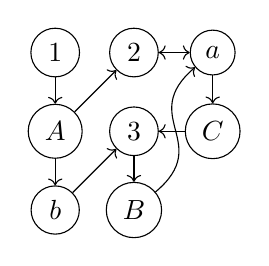
\begin{tikzpicture}[main/.style = {draw, circle}] 
         \node[main] at (0, 2) (1) {$1$}; 
         \node[main] at (0, 0) (b) {$b$};
         \node[main] at (0, 1) (A) {$A$};
        \node[main] at (2, 1) (C) {$C$};
        \node[main] at (2, 2) (a) {$a$};
        \node[main] at (1, 2) (2) {$2$};
        \node[main] at (1, 0) (B) {$B$};
        %\node[main] at (1, 0) (b) {$b$};
        \node[main] at (1, 1) (3) {$3$};
        \draw[->] (1) -- (A);
        \draw[->] (A) -- (b);
        \draw[->] (A) -- (2);
        \draw[->] (b) -- (3);
        \draw[<->] (2) -- (a);
        \draw[->] (a) -- (C);
        \draw[->] (C) -- (3);
        \draw[->] (3) -- (B);
        \draw[->] (B) to [out=40,in=220,looseness=1.5] (a);
        \end{tikzpicture}\caption{Type I-III-IC Graph}
        \end{subfigure}\hfill  
        \caption{Configuration with ESS and Bidirectional Output}\label{fig:ESS_Out_summary}
\end{figure} 
\section{Conclusion}
In this paper, an algorithm is developed, aiming to automate the PFG design process for Three-Port DC-DC power converters. The methods for translating the problem to a language understandable by a PC, validating the generated PFGAMs and placing the FCs in PFGs are properly described and the corresponding algorithm is presented in the form of pseudocode. Subsequently, a case study and several generated results (PFGAMs and graphs) are presented and discussed. Throughout this study, its contribution on the field is highlighted, as it does not only sets the PFG design methodology in a structured way, but also releases it from the restrictions and the toil associated with the manual derivation process. In future works, additional processing steps should be added after this algorithm to include optimization studies based on specific parameters, i.e. voltage gain and efficiency, and/or discover the most fitting power converter topologies for the FCs that consist the TPC converter.
\\
\\
\\
\\

\printbibliography
\end{document}
